\documentclass[10pt,letterpaper]{article}
\usepackage[margin=.66in,headheight=14pt,footskip=.34in]{geometry}
\usepackage[T1]{fontenc}
\usepackage{lmodern,microtype,amsmath,amssymb,mathtools,booktabs,array,multicol,enumitem,xcolor,tikz,fancyhdr,lastpage,needspace}
\usepackage[hidelinks,bookmarksnumbered=true]{hyperref}
\usetikzlibrary{arrows.meta,calc,positioning,angles,quotes}
\definecolor{solveRed}{RGB}{171,26,40}
\definecolor{navy}{RGB}{21,50,78}
\definecolor{muted}{RGB}{70,79,92}
\definecolor{soft}{RGB}{239,243,247}
\color{black}
\setlength{\parindent}{0pt}
\setlength{\parskip}{4pt}
\setlength{\abovedisplayskip}{5pt}
\setlength{\belowdisplayskip}{5pt}
\setlength{\abovedisplayshortskip}{3pt}
\setlength{\belowdisplayshortskip}{3pt}
\renewcommand{\arraystretch}{1.16}
\allowdisplaybreaks
\emergencystretch=2em
\pagestyle{fancy}\fancyhf{}
\fancyhead[L]{\footnotesize\bfseries CS 532 \textbar{} Quizzes by Lecture}
\fancyhead[R]{\footnotesize\color{muted}Lectures 1--6 \textbar{} red = numbered solution}
\fancyfoot[L]{\scriptsize\color{muted}Original quiz data preserved; supplemental explanations marked}
\fancyfoot[R]{\scriptsize Page \thepage\ of \pageref{LastPage}}
\renewcommand{\headrulewidth}{.3pt}
\newcounter{workedstep}
\newenvironment{steps}{\par\begingroup\color{solveRed}\setcounter{workedstep}{0}\small\setlength{\parskip}{4pt}}{\par\endgroup}
\newcommand{\Step}[1]{\par\refstepcounter{workedstep}\noindent\textbf{Step \arabic{workedstep}.}\ #1\par}
\newcommand{\Q}[2]{\par\Needspace{6\baselineskip}{\color{navy}\bfseries #1.}\ \textbf{#2}\par}
\newcommand{\Given}[1]{\par{\color{muted}\small\textbf{Given / relevant facts:} #1}\par}
\newcommand{\ExamNote}[1]{\par\begingroup\color{muted}\small\textbf{Exam check / qualification.} #1\par\endgroup}
\newcommand{\Final}[1]{\fbox{$\displaystyle #1$}}
\newcommand{\Quiz}[5]{\phantomsection\subsection*{#3\hfill\normalsize #4/100}\addcontentsline{toc}{subsection}{#3 (#4/100)}\label{quiz:#1}\noindent\textbf{Source:} \path{#2}\\\textbf{Lecture match:} #5\par\vspace{4pt}\hrule\vspace{5pt}}
% All figure labels and geometries are illustrative, not inferred camera measurements.
\newcommand{\EpipolarDiagram}{%
\begin{center}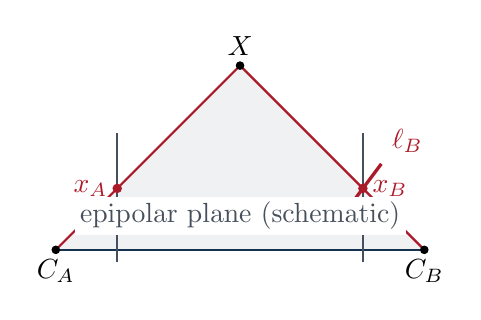
\begin{tikzpicture}[scale=.78,>=Stealth]
\coordinate (CA) at (0,0); \coordinate (CB) at (6,0); \coordinate (X) at (3,3);
\fill[navy!7] (CA)--(CB)--(X)--cycle;
\draw[navy,thick] (CA)--(CB); \draw[solveRed,thick] (CA)--(X)--(CB);
\draw[muted,thick] (1,-.2)--(1,1.9); \draw[muted,thick] (5,-.2)--(5,1.9);
\coordinate (a) at (1,1); \coordinate (b) at (5,1);
\fill (CA) circle (2pt) node[below]{$C_A$}; \fill (CB) circle (2pt) node[below]{$C_B$};
\fill (X) circle (2pt) node[above]{$X$};
\fill[solveRed] (a) circle (2.2pt) node[left]{$x_A$};
\fill[solveRed] (b) circle (2.2pt) node[right]{$x_B$};
\draw[solveRed,very thick] (4.7,.6)--(5.3,1.4) node[above right]{$\ell_B$};
\node[muted,fill=white,inner sep=2pt] at (3,.55){epipolar plane (schematic)};
\end{tikzpicture}\end{center}
\ExamNote{The 2D drawing is a cross-section of the epipolar plane. The actual epipolar line is the intersection of that 3D plane with image plane B; its apparent slant in the sketch is illustrative.}}
\newcommand{\FOVDiagram}{%
\begin{center}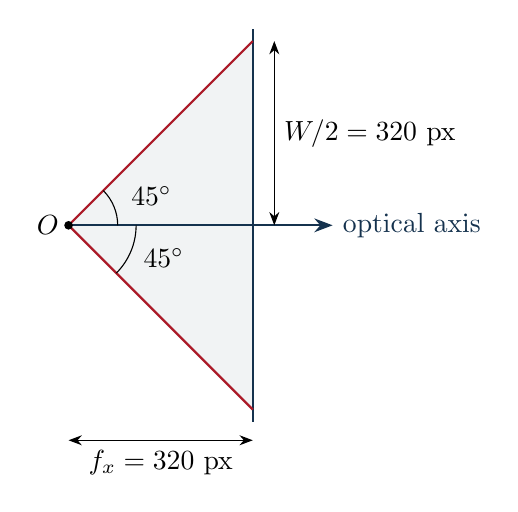
\begin{tikzpicture}[scale=.78,>=Stealth]
\coordinate (O) at (0,0); \coordinate (T) at (3,3); \coordinate (B) at (3,-3);
\fill[navy!6] (O)--(T)--(B)--cycle;
\draw[navy,thick,->] (O)--(4.3,0) node[right]{optical axis};
\draw[navy,thick] (3,-3.2)--(3,3.2);
\draw[solveRed,thick] (O)--(T) (O)--(B);
\draw (0.8,0) arc[start angle=0,end angle=45,radius=.8];
\draw (1.1,0) arc[start angle=0,end angle=-45,radius=1.1];
\node at (1.35,.48){$45^\circ$}; \node at (1.55,-.53){$45^\circ$};
\draw[<->] (3.35,0)--(3.35,3) node[midway,right]{$W/2=320$ px};
\draw[<->] (0,-3.5)--(3,-3.5) node[midway,below]{$f_x=320$ px};
\fill (O) circle(2pt) node[left]{$O$};
\end{tikzpicture}\end{center}}
\newcommand{\PosePlaneDiagram}{%
\begin{center}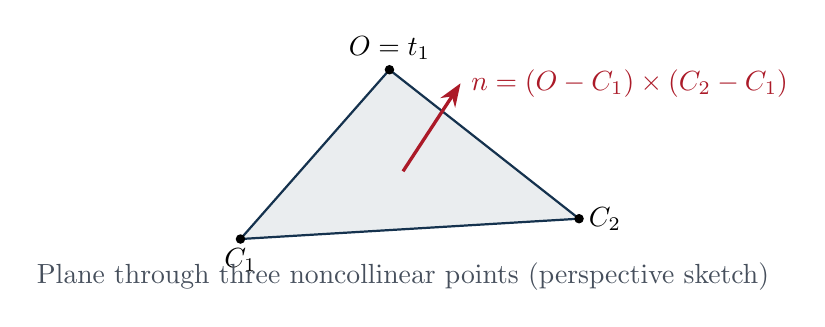
\begin{tikzpicture}[scale=.86,>=Stealth]
\coordinate (A) at (0,0); \coordinate (B) at (5,.3); \coordinate (C) at (2.2,2.5);
\fill[navy!9] (A)--(B)--(C)--cycle;
\draw[navy,thick] (A)--(B)--(C)--cycle;
\fill (A) circle(2pt) node[below]{$C_1$}; \fill (B) circle(2pt) node[right]{$C_2$};
\fill (C) circle(2pt) node[above]{$O=t_1$};
\draw[solveRed,very thick,->] (2.4,1)--(3.25,2.3) node[right]{$n=(O-C_1)\times(C_2-C_1)$};
\node[muted] at (2.4,-.55){Plane through three noncollinear points (perspective sketch)};
\end{tikzpicture}\end{center}}
\newcommand{\TetraDiagram}{%
\begin{center}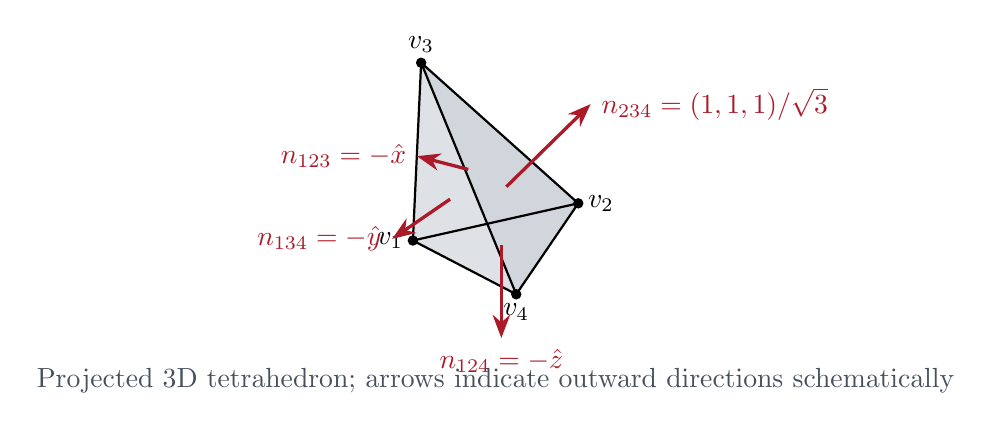
\begin{tikzpicture}[scale=1.05,>=Stealth]
% Affine projection of local coordinates (x-1,y-1,z) into drawing coordinates.
\coordinate (V1) at (0,0); \coordinate (V2) at (2.0,.45);
\coordinate (V3) at (.1,2.15); \coordinate (V4) at (1.25,-.65);
\fill[navy!7] (V1)--(V2)--(V3)--cycle;
\fill[navy!14] (V1)--(V3)--(V4)--cycle;
\fill[navy!20] (V2)--(V3)--(V4)--cycle;
\draw[thick] (V1)--(V2)--(V3)--cycle (V1)--(V4)--(V3) (V2)--(V4);
\foreach \p/\lab/\pos in {V1/v_1/left,V2/v_2/right,V3/v_3/above,V4/v_4/below}{\fill (\p) circle(1.8pt) node[\pos]{$\lab$};}
\draw[solveRed,very thick,->] (.67,.86)--(.05,1.02) node[left]{$n_{123}=-\hat x$};
\draw[solveRed,very thick,->] (1.07,-.06)--(1.07,-1.18) node[below]{$n_{124}=-\hat z$};
\draw[solveRed,very thick,->] (.45,.5)--(-.25,.02) node[left]{$n_{134}=-\hat y$};
\draw[solveRed,very thick,->] (1.13,.65)--(2.15,1.65) node[right]{$n_{234}=(1,1,1)/\sqrt3$};
\node[muted] at (1,-1.7){Projected 3D tetrahedron; arrows indicate outward directions schematically};
\end{tikzpicture}\end{center}}
\newcommand{\repeatnote}[1]{{\color{muted}\small\textit{Near duplicate: #1}}\par}
\begin{document}
\begin{titlepage}
\centering\vspace*{1.1in}
{\color{navy}\Huge\bfseries CS 532\\[8pt] 18 Quizzes --- Organized by Lecture}\par\vspace{.3in}
{\Large Exam-reference edition}\par\vspace{.4in}
{\large Each original question and subquestion, with \textcolor{solveRed}{numbered red steps}, substitutions, equations, verified answers, and completed diagrams.}\par\vspace{.7in}
\begin{minipage}{.82\linewidth}
\textbf{Scope:} The 18 quizzes supplied in the source guide, grouped by primary lecture match (Lectures 1--6). The original relevance scores and duplicates are preserved; two additional quizzes mentioned in the study outline were not supplied and are not invented.\par\medskip
\textbf{Conventions:} Image points are homogeneous unless otherwise indicated. A virtual image plane lies at camera $z=f$ for pinhole derivations. Camera/world transformation direction is always specified explicitly.\par\medskip
\textbf{How to use during an exam:} Use the lecture sections, contents page, quiz title, or formula locator. In every problem, the question is in black, the complete method is \textcolor{solveRed}{red}, and important caveats are gray.\par\medskip
\textbf{Source fidelity:} The question statements follow the uploaded old quiz PDFs (edited slightly for typography/clarity but never changing numerical givens). Where the supplied Fall 2025 answer key uses ambiguous or inaccurate notation, a clearly labeled check follows it. Additional example calculations appear only when labeled \emph{illustrative}.\par
\end{minipage}
\vfill
{\color{muted}\large CS 532 \textbar{} Lectures 1--6 \textbar{} Study copy}\par
\end{titlepage}
\tableofcontents\clearpage
\section*{Lecture organization and score legend}\addcontentsline{toc}{section}{Lecture organization and score legend}
\textbf{Primary lecture match:} Every quiz appears once, under its principal lecture. Secondary lecture overlaps are mentioned in section study notes.\par
\textbf{Relevance grades:} A = highest relevance; B = strong relevance; C = partial relevance; D = outside the six-lecture scope. The numerical scores shown in quiz headings are \emph{relevance scores, not grades on the worked solutions}.\par
\textbf{Count clarification:} The supplied outline says ``20 quizzes,'' but the six tables list 18 entries, matching the 18 quizzes in this source. This edition therefore includes 18 historical quizzes plus seven clearly labeled original practice problems.\par
\medskip
\section*{Fast formula locator}\addcontentsline{toc}{section}{Fast formula locator}
\begin{tabular}{@{}p{.28\linewidth}p{.65\linewidth}@{}}
\toprule
\textbf{Concept} & \textbf{Core relation / worked quizzes}\\\midrule
Epipolar geometry & $\ell'=Fx$, $x'^TFx=0$, $e'^TF=0$; Lecture 4\\
Stereo geometry & $Z=bf/d$, $\Delta Z\approx-bf\,\Delta d/d^2$; Lecture 4\\
Homography/RANSAC & $x'\sim Hx$, $N\geq\ln(1-p)/\ln(1-w^s)$; Lecture 3\\
Projective primitives & $\ell=a\times b$, $c^T\ell=0$; Lecture 2\\
KLT brightness & $I_xu+I_yv+I_t=0$; Lecture 5\\
Camera geometry & $x\sim K[R\mid t]X$, $f_x=(W/2)/\tan(\theta/2)$; Lecture 3\\
SfM & Gauge, plane at infinity, incremental reconstruction, bundle adjustment; Lecture 6\\
Harris & $M=\sum w\nabla I\nabla I^T$, $R=\det M-k(\operatorname{tr}M)^2$; Lecture 5\\
Rigid geometry & Pose composition, plane normals, $R_z(90^\circ)$; Lecture 1\\
\bottomrule
\end{tabular}
\vspace{10pt}
\textbf{Key unit warning:} In $Z=bf/d$, $b$ and $Z$ have the same physical units; $f$ and $d$ use the same image-coordinate units (usually pixels). Distinguish \emph{exact} depth error from the \emph{first-order} Taylor approximation.\par
\textbf{Common symbol warning:} $Fx$ and $F^Tx'$ are \emph{line coefficient vectors}, not generally pixel coordinates. A line $\ell=(a,b,c)^T$ means $au+bv+c=0$ for image coordinates $(u,v)$.\par

\clearpage\phantomsection\section*{Lecture 1 --- Foundations and 3D Geometry}\addcontentsline{toc}{section}{Lecture 1 --- Foundations and 3D Geometry}\label{lecture:1}
\textbf{Lecture study note.} Supplementary practice: camera-relative poses, 3D planes, depth-map backprojection and surface normals. Also relevant to Lectures 3--4.\par
\textbf{Relevance scores in this section are from the original quiz-matching rubric, not solution grades.}
% QUIZ 17
\Quiz{17}{cs532f25_quiz_1_solution.pdf}{Fall 2025 Quiz 1 --- Probability and rigid camera poses}{69}{Lectures 1--4; RANSAC probability analogy}
\Q{Question 1}{A parlay succeeds only if all three independent fair coin flips succeed. What is the chance of winning one parlay?}
\begin{steps}
\Step{Each fair flip succeeds with probability $1/2$. The three flip outcomes are independent.}
\Step{Multiply probabilities for the joint event: $P(\text{all 3})=(1/2)^3=1/8$.}
\Step{$\boxed{P(\text{win})=1/8=12.5\%}$. This is the same product rule used for all-inlier RANSAC samples.}
\end{steps}
\Q{Question 2}{You attempt one three-coin-flip parlay each day for seven independent days. What is the probability of winning at least one?}
\begin{steps}
\Step{One parlay win probability is $q=1/8$. Its loss probability is $1-q=7/8$.}
\Step{All seven attempts fail with probability $P(0\text{ wins})=(7/8)^7$.}
\Step{Use the complement of no wins: \[P(\ge1\text{ win})=1-(7/8)^7=1-823543/2097152.\]}
\Step{Therefore $\boxed{P(\ge1\text{ win})\approx0.607304\approx60.73\%}$.}
\end{steps}
\Q{Question 3}{Two static cameras concurrently estimate the 3D rigid pose of the same object, as $[R_1,t_1]$ and $[R_2,t_2]$ in their own camera frames. Can one recover the relative camera pose? Explain and derive a transformation.}
\begin{steps}
\Step{Define $^{C_i}T_O=\begin{bmatrix}R_i&t_i\\0&1\end{bmatrix}$, which maps an object-frame homogeneous point $X_O$ into camera frame $C_i$: $X_{C_i}={}^{C_i}T_O X_O$. Both poses refer to the \emph{same object at the same time}.}
\Step{Express the object coordinates from camera-2 coordinates: $X_O=({}^{C_2}T_O)^{-1}X_{C_2}$.}
\Step{Insert into camera-1 expression: $X_{C_1}={}^{C_1}T_O({}^{C_2}T_O)^{-1}X_{C_2}$.}
\Step{Thus $\boxed{{}^{C_1}T_{C_2}={}^{C_1}T_O({}^{C_2}T_O)^{-1}}$. The inverse gives $^{C_2}T_{C_1}$.}
\Step{Expand if asked: inverse of $[R_2,t_2]$ is $[R_2^T,-R_2^Tt_2]$; therefore $R_{12}=R_1R_2^T$, $t_{12}=t_1-R_1R_2^Tt_2$.}
\end{steps}
\ExamNote{The uploaded key's superscript/subscript arrows are inconsistent in places. The formula above is unambiguous because its mapping direction is defined explicitly. If the poses are only known up to unknown scale, relative metric translation is not determined absolutely.}
\Q{Question 4}{Can one determine the 3D plane passing through both camera centers and the tracked object's center? Derive it.}
\begin{steps}
\Step{Use camera-1 coordinates as the world frame: $C_1=(0,0,0)^T$. The object-frame origin is observed at $O=t_1$.}
\Step{Find camera-2 center $C_2$ as the translation part of the transform $^{C_1}T_{C_2}$ from Question 3.}
\Step{Two vectors lying in the plane are $a=O-C_1$ and $b=C_2-C_1$. Take the cross product to find a plane normal: $\boxed{n=a\times b}$.}
\Step{The plane equation is $n^T(X-C_1)=0$ or $n^TX+d=0$ with $d=-n^TC_1$. Because $C_1=0$, $\boxed{n^TX=0}$.}
\Step{Require $n\ne0$, i.e. the three points are noncollinear. If cameras and object center lie on one line, infinitely many planes contain them. Draw a triangle joining $C_1,C_2,O$ with a perpendicular arrow $n$.}
\end{steps}
\PosePlaneDiagram

\clearpage
% QUIZ 18
\Quiz{18}{cs532_f17_quiz9.pdf}{Fall 2017 Quiz 9 --- Depth maps and tetrahedron normals}{55}{Lectures 1--4 transfer; normals/point-cloud topics are only partly in scope}
\Q{Problem 1}{Explain how to convert two depth maps into a single 3D point cloud in a common reference frame. What information is required? Make a sketch.}
\begin{steps}
\Step{For camera $i\in\{1,2\}$ obtain intrinsic matrix $K_i$, per-pixel depth $Z_i(u,v)$, and a known camera-to-world rigid transform $^{W}T_{C_i}=\begin{bmatrix}R_i&t_i\\0&1\end{bmatrix}$. First correct lens distortion if depth is reported in distorted coordinates.}
\Step{For pixel $p_i=(u,v,1)^T$, compute normalized camera ray $r_i=K_i^{-1}p_i$, whose last component is 1 under standard intrinsics. If depth means camera-axis $Z$, backproject: $\boxed{X_{C_i}=Z_i(u,v)\,K_i^{-1}p_i}$.}
\Step{For standard intrinsics with zero skew this becomes $X_{C_i}=((u-c_x)Z/f_x,(v-c_y)Z/f_y,Z)^T$. Skip missing, zero, invalid, or occluded depth pixels.}
\Step{Map every 3D point into the \emph{same} world frame: $\boxed{X_W=R_iX_{C_i}+t_i}$. Combine both transformed sets; optional voxel fusion/outlier removal prevents duplicates or inconsistent observations.}
\Step{If depth means \emph{Euclidean range along ray}, use $X_{C_i}=\rho_i r_i/\|r_i\|$, not $Z_i r_i$. The question needs a depth convention, the two sets of intrinsics, and the relative/world poses.}
\end{steps}
\begin{center}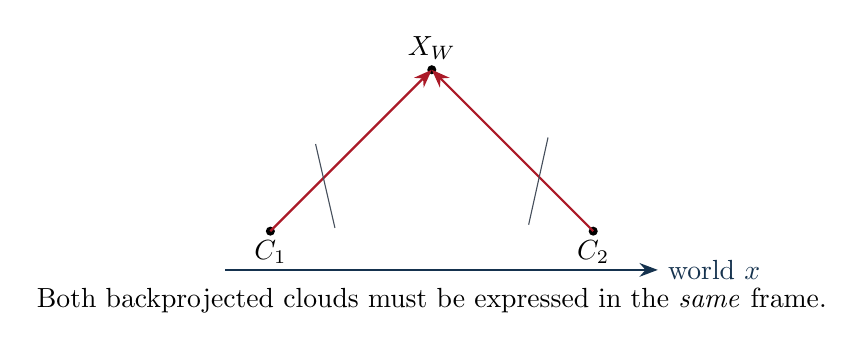
\begin{tikzpicture}[scale=.82,>=Stealth]
\coordinate (C1) at (0,0);\coordinate (C2) at (5,0);\coordinate (X) at (2.5,2.5);
\draw[navy,thick,->] (-.7,-.6)--(6,-.6) node[right]{world $x$};
\fill (C1) circle(2pt) node[below]{$C_1$};\fill (C2) circle(2pt) node[below]{$C_2$};\fill (X) circle(2pt) node[above]{$X_W$};
\draw[solveRed,thick,->] (C1)--(X);\draw[solveRed,thick,->] (C2)--(X);
\draw[muted] (1.0,.05)--(.7,1.35);\draw[muted] (4,.1)--(4.3,1.45);
\node at (2.5,-1.08){Both backprojected clouds must be expressed in the \emph{same} frame.};
\end{tikzpicture}\end{center}
\Q{Problem 2(a)}{A tetrahedron has vertices $v_1=(1,1,0)$, $v_2=(1,2,0)$, $v_3=(1,1,1)$, $v_4=(2,1,0)$. Find one \emph{outward} surface normal per face, and sketch the result.}
\begin{steps}
\Step{Choose the four triangular faces: $(1,2,3)$, $(1,2,4)$, $(1,3,4)$, and $(2,3,4)$. For vertices $i,j,k$, calculate candidate $n_{ijk}=(v_j-v_i)\times(v_k-v_i)$.}
\Step{Face 123: $v_2-v_1=(0,1,0)$ and $v_3-v_1=(0,0,1)$; cross product gives $(1,0,0)$. Since the opposite vertex $v_4$ has $x=2$, interior points face +x, so outward normal is $\boxed{n_{123}=(-1,0,0)}$.}
\Step{Face 124: $v_2-v_1=(0,1,0)$, $v_4-v_1=(1,0,0)$; cross product is $(0,0,-1)$, pointing away from opposite $v_3$ above $z=0$. Thus $\boxed{n_{124}=(0,0,-1)}$.}
\Step{Face 134: $v_3-v_1=(0,0,1)$, $v_4-v_1=(1,0,0)$; cross product $(0,1,0)$ points toward opposite $v_2$ with $y=2$. Flip: $\boxed{n_{134}=(0,-1,0)}$.}
\Step{Face 234: $v_3-v_2=(0,-1,1)$ and $v_4-v_2=(1,-1,0)$. Cross product $(1,1,1)$, which points away from opposite vertex $v_1$ across plane $x+y+z=3$. Thus $\boxed{n_{234}=(1,1,1)/\sqrt3}$ for a unit normal.}
\Step{Sketch triangular faces forming the tetrahedron and draw the four arrows perpendicular to their face planes, directed away from its interior. The first three have unit magnitude already; the fourth needs division by $\sqrt3$ for unit length.}
\end{steps}
\TetraDiagram
\Q{Problem 2(b)}{Rotate the complete tetrahedron by $+90^\circ$ about the global $Z$ axis. Find the modified face normals.}
\begin{steps}
\Step{For an \emph{active}, right-handed $+90^\circ$ rotation, \[R_z(90^\circ)=\begin{bmatrix}\cos90^\circ&-\sin90^\circ&0\\\sin90^\circ&\cos90^\circ&0\\0&0&1\end{bmatrix}=\begin{bmatrix}0&-1&0\\1&0&0\\0&0&1\end{bmatrix}.\]}
\Step{Pure rigid rotations rotate normals by the same matrix: $n'_{ijk}=R_zn_{ijk}$. (General nonrigid affine transforms use an inverse-transpose rule instead.)}
\Step{Compute each: $R_z(-1,0,0)^T=(0,-1,0)^T$; $R_z(0,0,-1)^T=(0,0,-1)^T$; $R_z(0,-1,0)^T=(1,0,0)^T$.}
\Step{For the slanted face, $R_z(1,1,1)^T/\sqrt3=(-1,1,1)^T/\sqrt3$.}
\Step{Collect the results: \[\boxed{n'_{123}=(0,-1,0),\quad n'_{124}=(0,0,-1),}\]\[\boxed{n'_{134}=(1,0,0),\quad n'_{234}=(-1,1,1)/\sqrt3.}\]}
\end{steps}

\clearpage\phantomsection\section*{Lecture 2 --- Projective Geometry and Linear Algebra}\addcontentsline{toc}{section}{Lecture 2 --- Projective Geometry and Linear Algebra}\label{lecture:2}
\textbf{Lecture study note.} Coverage gap: advanced rotation representations, quaternions and transformation hierarchies are not directly tested by these historical quizzes. Also relevant to Lecture 1.\par
\textbf{Relevance scores in this section are from the original quiz-matching rubric, not solution grades.}
% QUIZ 8
\Quiz{8}{cs532s20_quiz1.pdf}{Spring 2020 Quiz 1 --- Projective points and camera projection}{96}{Lectures 1--2}
\Q{Problem 1}{For projective-plane points $a,b,c$, use only dot and cross products to test whether they are collinear. In what case does the test fail?}
\begin{steps}
\Step{Recall that the homogeneous \emph{line through two distinct points} is their cross product: $\ell=a\times b$.}
\Step{A third point $c$ lies on $\ell$ exactly when its dot product with $\ell$ is zero. Thus test $\boxed{c^T(a\times b)=0}$. This equals the determinant of the matrix with columns $a,b,c$.}
\Step{Check degeneracy: if $a\sim b$ (they represent the same projective point), then $a\times b=0$, and the test returns zero for \emph{every} $c$, including noncollinear ones. Use a different pair of distinct representatives if possible. The zero homogeneous vector is invalid as a point.}
\end{steps}
\Q{Problem 2(a--b)}{Let $X=(X,Y,Z,W)^T$ be a homogeneous 3D point and $x\sim MX$ a homogeneous 2D image point. Find (a) the dimensions of $M$; (b) explicit inhomogeneous image coordinates from the entries $m_{ij}$ and $X$.}
\begin{steps}
\Step{A 3D homogeneous point has four components; a 2D homogeneous image point has three. Therefore $\boxed{M\in\mathbb R^{3\times4}}$ and $Mx\!$ is \emph{not} the mapping; the correct product is $MX\in\mathbb R^{3\times1}$.}
\Step{Write $M=[m_{ij}]$ and compute $q=MX=(q_1,q_2,q_3)^T$ with $q_i=m_{i1}X+m_{i2}Y+m_{i3}Z+m_{i4}W$.}
\Step{Convert homogeneous to inhomogeneous coordinates by dividing by the third component: \[\boxed{u=\frac{m_{11}X+m_{12}Y+m_{13}Z+m_{14}W}{m_{31}X+m_{32}Y+m_{33}Z+m_{34}W}},\quad\boxed{v=\frac{m_{21}X+m_{22}Y+m_{23}Z+m_{24}W}{m_{31}X+m_{32}Y+m_{33}Z+m_{34}W}}.\] For ordinary 3D coordinates set $W=1$; require $q_3\ne0$ to get a finite pixel.}
\end{steps}
\Q{Problem 3(a--b)}{Let $\ell_1,\ell_2$ be two distinct vertical lines each at distance $d>0$ from the 2D origin, and $\ell_3$ the horizontal line through the origin. Give their homogeneous line vectors and count the possible pairwise intersections.}
\begin{steps}
\Step{Choose $\ell_1:x=d$ and $\ell_2:x=-d$; as $ax+by+c=0$, their vectors are $\boxed{\ell_1=(1,0,-d)^T}$, $\boxed{\ell_2=(1,0,d)^T}$.}
\Step{For the horizontal line $y=0$, use $\boxed{\ell_3=(0,1,0)^T}$. Line vectors are homogeneous, so nonzero multiples are equivalent.}
\Step{Intersect $\ell_1,\ell_3$: $\ell_1\times\ell_3=(d,0,1)^T\Rightarrow\boxed{(d,0)}$. Intersect $\ell_2,\ell_3$: $\ell_2\times\ell_3=(-d,0,1)^T\Rightarrow\boxed{(-d,0)}$.}
\Step{Intersect the \emph{parallel} vertical lines: $\ell_1\times\ell_2=(0,-2d,0)^T\sim(0,1,0)^T$, a \emph{point at infinity}, not a finite 2D coordinate.}
\Step{Thus $\boxed{3\text{ projective intersections}}$ among the 3 line pairs, of which $\boxed{2\text{ are finite}}$. Say both numbers to clarify the geometric convention.}
\end{steps}

\clearpage\phantomsection\section*{Lecture 3 --- Camera Projection, Homographies, and RANSAC}\addcontentsline{toc}{section}{Lecture 3 --- Camera Projection, Homographies, and RANSAC}\label{lecture:3}
\textbf{Lecture study note.} Spring 2019 Quiz 2 and Spring 2020 Quiz 3 are near-duplicates. Coverage gaps: numerical DLT, SVD, normalized homography estimation and image warping. The supplement provides DLT/SVD practice. Secondary overlaps: Lectures 1--2.\par
\textbf{Relevance scores in this section are from the original quiz-matching rubric, not solution grades.}
% QUIZ 7
\Quiz{7}{cs532s19-quiz3.pdf}{Spring 2019 Quiz 3 --- Pentagon, homography, RANSAC}{97}{Lecture 3, slides 34--55}
\Q{Problem 1(a--d)}{Two images show only the same \emph{irregular five-sided polygon}, related by an unknown homography. All five corners are detected in each image. You create every possible putative corner correspondence. (a) How many? (b) What inlier rate? (c) How many RANSAC iterations are needed to reliably estimate the homography? (d) What changes for a regular/equilateral pentagon?}
\begin{steps}
\Step{There are 5 features in image A and 5 in image B. Exhaustive matching forms all ordered cross-image pairs, so $\boxed{5\times5=25}$ putative correspondences.}
\Step{Assume one unique correct correspondence for each of the 5 image-A corners. Then 5 of the 25 pairs are inliers, so $\boxed{w=5/25=0.2}$ and outlier rate $e=0.8$.}
\Step{The minimal homography solver requires $s=4$ nondegenerate correspondences. The usual RANSAC independent-sample approximation sets \[1-(1-w^s)^N\ge p\quad\Rightarrow\quad N\ge\frac{\ln(1-p)}{\ln(1-w^s)}.\]}
\Step{For the \emph{illustrative} common confidence $p=0.99$, $w^4=0.2^4=0.0016$, hence \[\boxed{N_{\mathrm{approx}}=\left\lceil\frac{\ln(0.01)}{\ln(0.9984)}\right\rceil=2876}.\] The quiz does not specify a confidence; the general formula is the source-supported answer. Sampling all putative matches independently also ignores the one-to-one matching constraint, so these iteration counts describe a simplified model.}
\Step{Because there are only 25 candidate pairs and each RANSAC \emph{sample selects 4 distinct pairs}, the exact probability of four inliers in a uniform draw without replacement is smaller: \[q_{\mathrm{exact}}=\frac{\binom54}{\binom{25}4}=\frac5{12650}\approx0.00039526.\] If \emph{each trial samples afresh} and we desire $p=0.99$, \[\boxed{N_{\mathrm{finite}}=\left\lceil\frac{\ln(.01)}{\ln(1-5/12650)}\right\rceil=11649}.\] This is an optional exact finite-population refinement; the standard lecture approximation uses $w^s$.}
\Step{For a regular pentagon, rotational/reflection symmetry makes the corner identities ambiguous: several match permutations may fit geometrically similar configurations. Without texture/orientation/other cues, a unique physical correspondence is less secure. Explain that good geometric fits need not identify the \emph{intended} corner labeling.}
\end{steps}
\ExamNote{The irregular-pentagon problem still requires nondegenerate 4-tuples (e.g. no three source points collinear). The exact without-replacement refinement above does not imply that \emph{every} four-inlier subset yields a uniquely acceptable model under all degeneracies.}

\clearpage
% QUIZ 10
\Quiz{10}{cs532s19_quiz2-2.pdf}{Spring 2019 Quiz 2 --- FOV, calibration, homogeneous scaling}{93}{Lectures 1--3}
\Q{Problem 1}{A digital camera has image resolution $640\times480$ pixels and horizontal field of view $90^\circ$. Determine the focal length in pixels and draw a sketch.}
\begin{steps}
\Step{Take a horizontal cross-section through the optical axis. The full horizontal FOV is $90^\circ$, so each edge ray is $45^\circ$ from the optical axis. The image half-width is $W/2=320$ pixels.}
\Step{In the pinhole triangle, $\tan(\theta/2)=(W/2)/f_x$. Rearrange: $f_x=(W/2)/\tan(\theta/2)$.}
\Step{Substitute $W=640$, $\theta=90^\circ$: \[\boxed{f_x=\frac{320}{\tan45^\circ}=320\ \mathrm{px}}.\]}
\end{steps}
\FOVDiagram
\Q{Problem 2}{Write the intrinsic calibration matrix $K$ for the camera.}
\begin{steps}
\Step{Use standard intrinsic form $K=\begin{bmatrix}f_x&s&c_x\\0&f_y&c_y\\0&0&1\end{bmatrix}$.}
\Step{The horizontal FOV determines $f_x=320$ px only. To fill the other terms, \emph{assume} square pixels ($f_y=f_x$), zero skew ($s=0$), and centered principal point ($(c_x,c_y)=(320,240)$).}
\Step{Under those common assumptions, \[\boxed{K=\begin{bmatrix}320&0&320\\0&320&240\\0&0&1\end{bmatrix}}.\] Without them, $f_y,s,c_x,c_y$ cannot all be inferred from the given horizontal FOV alone.}
\end{steps}
\Q{Problem 3(a--b)}{In $x=K[R\mid t]X$, give dimensions of every matrix/vector. If the right-hand side is multiplied by 2 to obtain $x'=2K[R\mid t]X$, how are $x'$ and $x$ related?}
\begin{steps}
\Step{$K:3\times3$, $R:3\times3$, $t:3\times1$, $[R\mid t]:3\times4$, $X:4\times1$, $x:3\times1$; total projection matrix $P=K[R\mid t]$ is $3\times4$.}
\Step{Homogeneous images are defined up to nonzero scale: $x'=(2q_1,2q_2,2q_3)^T$ vs $x=(q_1,q_2,q_3)^T$.}
\Step{Dehomogenize: $u'=2q_1/(2q_3)=q_1/q_3=u$ and $v'=2q_2/(2q_3)=v$. So $\boxed{x'\sim x}$: identical physical image points.}
\end{steps}
\Q{Problem 4}{What are the 3D coordinates of the image principal point in the camera coordinate system?}
\begin{steps}
\Step{The principal point is the intersection of the camera optical axis with the image plane. In a virtual plane $z=f_{\mathrm{physical}}$, the optical axis is $X=Y=0$.}
\Step{Therefore its camera-frame position is $\boxed{(0,0,f_{\mathrm{physical}})}$. If the image-plane coordinate units are \emph{chosen as pixel-equivalent units}, one may write $(0,0,320)$ using the computed focal length in pixels.}
\Step{Distinguish this 3D position from the image-array pixel coordinates $\boxed{(c_x,c_y)=(320,240)}$ under the centered-principal-point assumption. Physical $f$ in meters/mm is not determined by pixel focal length alone without pixel pitch.}
\end{steps}

\clearpage
% QUIZ 11
\Quiz{11}{cs532s20_quiz3.pdf}{Spring 2020 Quiz 3 --- Duplicate camera model}{93}{Lectures 1--3}
\repeatnote{This PDF repeats rank 10's four camera-calibration questions; independent fully worked answers follow.}
\Q{Problem 1}{A camera is $640$ pixels wide by $480$ tall with horizontal FOV $90^\circ$. Find pixel focal length and sketch the rays.}
\begin{steps}
\Step{Half-angle is $90^\circ/2=45^\circ$, and half-width is $640/2=320$ pixels. Draw the camera center, optical axis and the rays to the two horizontal ends of the image plane.}
\Step{$\tan45^\circ=(320\,\mathrm{px})/f_x$.}
\Step{Since $\tan45^\circ=1$, $\boxed{f_x=320\,\mathrm{px}}$. The half-angle/FOV diagram on the preceding quiz applies.}
\end{steps}
\FOVDiagram
\Q{Problem 2}{Write the camera intrinsic matrix $K$.}
\begin{steps}
\Step{Use $K=\begin{bmatrix}f_x&s&c_x\\0&f_y&c_y\\0&0&1\end{bmatrix}$. The supplied FOV fixes only $f_x$.}
\Step{Explicitly assume square pixels $f_y=f_x=320$, zero skew $s=0$, and principal point at $(320,240)$.}
\Step{Then $\boxed{K=\begin{bmatrix}320&0&320\\0&320&240\\0&0&1\end{bmatrix}}$.}
\end{steps}
\Q{Problem 3(a--b)}{Give dimensions in $x=K[R\mid t]X$ and explain what doubling the full homogeneous right-hand side changes.}
\begin{steps}
\Step{Identify $K\in\mathbb R^{3\times3}$, $R\in\mathbb R^{3\times3}$, $t\in\mathbb R^{3\times1}$, $[R\mid t]\in\mathbb R^{3\times4}$, $X\in\mathbb R^{4\times1}$, $x\in\mathbb R^{3\times1}$.}
\Step{For projected $x=(a,b,c)^T$, the doubled homogeneous vector $x'=2x=(2a,2b,2c)^T$.}
\Step{The dehomogenized coordinates are the same: $(a/c,b/c)=(2a/2c,2b/2c)$. Answer: $\boxed{\text{no image location change}}$.}
\end{steps}
\Q{Problem 4}{Find the 3D coordinates of the principal point in the camera reference frame.}
\begin{steps}
\Step{Set the optical-axis ray to $\{(0,0,Z):Z>0\}$; intersect with virtual image plane $z=f_{\mathrm{physical}}$.}
\Step{The point is $\boxed{(0,0,f_{\mathrm{physical}})}$ in camera length units; in pixel-normalized plane units $f=320$ gives the coordinate triple $(0,0,320)$.}
\Step{If the question instead asks for image-array pixel coordinates, use $(c_x,c_y)=(320,240)$ under the stated centering assumption.}
\end{steps}

\clearpage
% QUIZ 14
\Quiz{14}{cs532s20_quiz2.pdf}{Spring 2020 Quiz 2 --- Pinhole ray and cross product}{90}{Lectures 2--3}
\Q{Problem 1}{Let $A=(X,Y,Z)$ be a camera-frame 3D point. Its viewing ray passes through image point $a$ on the image plane. Given $f=Z/10$, determine the 3D camera-frame coordinates of $a$; sketch.}
\begin{steps}
\Step{For a virtual pinhole image plane at $z=f$, the 3D point and pixel lie on the same ray from the origin. Similar triangles give $x_a/f=X/Z$ and $y_a/f=Y/Z$.}
\Step{Thus $a=(fX/Z,fY/Z,f)$.}
\Step{Substitute $f=Z/10$, assuming $Z\ne0$: \[\boxed{a=(X/10,Y/10,Z/10)=A/10}.\]}
\Step{Draw origin $O$, the point $A$, the intermediate image plane $z=f$, and $a$ on the segment of ray $OA$ (for $Z>0$ and $f=Z/10$). The vectors $Oa$ and $OA$ point in the same direction.}
\end{steps}
\begin{center}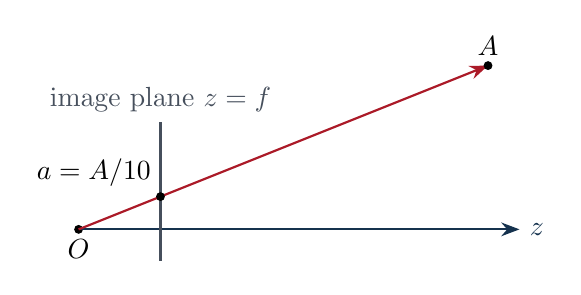
\begin{tikzpicture}[scale=.8,>=Stealth]
\fill (0,0) circle(2pt) node[below]{$O$};\draw[navy,thick,->] (0,0)--(7,0) node[right]{$z$};
\draw[muted,thick] (1.3,-.5)--(1.3,1.7) node[above]{image plane $z=f$};
\draw[solveRed,thick,->] (0,0)--(6.5,2.6);\fill (1.3,.52) circle(2pt) node[above left]{$a=A/10$};
\fill (6.5,2.6) circle(2pt) node[above]{$A$};
\end{tikzpicture}\end{center}
\Q{Problem 2}{Develop the expression for $A\times a$.}
\begin{steps}
\Step{Set $A=(X,Y,Z)^T$ and $a=(X/10,Y/10,Z/10)^T$.}
\Step{Use the cross-product determinant: \[A\times a=\begin{vmatrix}\mathbf i&\mathbf j&\mathbf k\\X&Y&Z\\X/10&Y/10&Z/10\end{vmatrix}.\]}
\Step{Expand components: $(YZ/10-ZY/10,\ ZX/10-XZ/10,\ XY/10-YX/10)$.}
\Step{Every component is zero, so $\boxed{A\times a=(0,0,0)^T}$. Geometrically, collinear vectors have zero cross product.}
\end{steps}

\clearpage
% QUIZ 15
\Quiz{15}{cs532f15_quiz9.pdf}{Older Quiz 9 --- Pinhole ray intersects a 3D plane}{88}{Lectures 2--3; source PDF header: Spring 2019 Quiz 9}
\Q{Problem 1}{A 3D plane has homogeneous parameters $\pi=(A,B,C,D)^T$, i.e. $AX+BY+CZ+D=0$. A pinhole camera has center at the 3D origin, orientation $I$, focal length $f$, and observes pixel image-plane coordinates $(x',y')$. Find the 3D depth of the intersection of the viewing ray with the plane. Draw a sketch.}
\begin{steps}
\Step{The ray begins at camera origin and passes through $(x',y',f)$ on the virtual image plane. Its parametric form is $r(\lambda)=\lambda(x',y',f)=(\lambda x',\lambda y',\lambda f)$.}
\Step{Using pinhole geometry, $x'/f=X/Z$, $y'/f=Y/Z$, hence $X=(x'/f)Z$ and $Y=(y'/f)Z$.}
\Step{Substitute into plane equation: \[A\frac{x'Z}{f}+B\frac{y'Z}{f}+CZ+D=0.\]}
\Step{Factor out $Z$: $Z(Ax'/f+By'/f+C)=-D$.}
\Step{Solve the optical-axis depth: \[\boxed{Z=-\frac{Df}{Ax'+By'+Cf}}.\]}
\Step{Recover the complete intersection point, if requested: \[\boxed{X=\frac{x'Z}{f},\quad Y=\frac{y'Z}{f},\quad Z=-\frac{Df}{Ax'+By'+Cf}}.\] Equivalently $\lambda=-D/(Ax'+By'+Cf)$ and $r(\lambda)$ gives all three coordinates.}
\Step{Check exceptions: if $Ax'+By'+Cf=0$ and $D\ne0$, the viewing ray is parallel to the plane (no finite intersection). If both equal zero, the entire ray lies in the plane (no unique depth). A visible front-of-camera intersection normally requires $Z>0$.}
\end{steps}
\begin{center}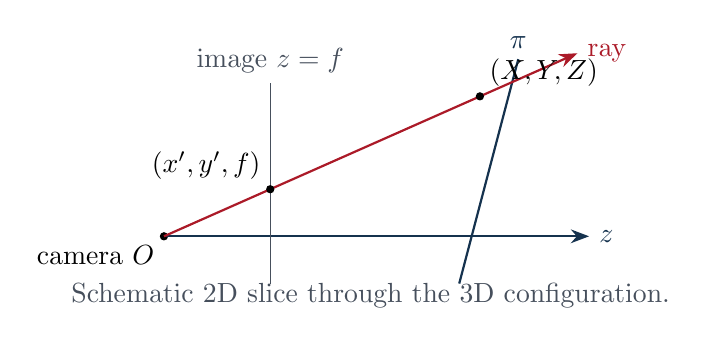
\begin{tikzpicture}[scale=.75,>=Stealth]
\fill (0,0) circle(2pt) node[below left]{camera $O$};\draw[navy,thick,->] (0,0)--(7.2,0) node[right]{$z$};
\draw[muted] (1.8,-.8)--(1.8,2.6) node[above]{image $z=f$};
\draw[navy,thick] (5,-.8)--(6,3) node[above]{$\pi$};
\draw[solveRed,thick,->] (0,0)--(7,3.1) node[right]{ray};
\fill (1.8,.797) circle(2pt) node[above left]{$(x',y',f)$};
\fill (5.35,2.37) circle(2pt) node[above right]{$(X,Y,Z)$};
\node[muted] at (3.5,-1){Schematic 2D slice through the 3D configuration.};
\end{tikzpicture}\end{center}
\ExamNote{The formula gives $Z$ (depth along optical axis), not necessarily Euclidean camera-to-point range $\sqrt{X^2+Y^2+Z^2}$.}

\clearpage\phantomsection\section*{Lecture 4 --- Two-View Geometry and Stereo}\addcontentsline{toc}{section}{Lecture 4 --- Two-View Geometry and Stereo}\label{lecture:4}
\textbf{Lecture study note.} Most heavily represented lecture. Duplicate pairs: 2015 Quiz 4 / Spring 2019 Quiz 4, and Spring 2019 Quiz 5 / Spring 2020 Quiz 5. Coverage gaps: essential-matrix decomposition, normalized eight-point estimation, triangulation and stereo matching costs. See supplemental examples.\par
\textbf{Relevance scores in this section are from the original quiz-matching rubric, not solution grades.}
% QUIZ 1
\Quiz{1}{cs532f15_quiz4.pdf}{Older Quiz 4 --- Epipolar line and constraint}{100}{Lecture 4, slides 18--21}
\Q{Problem 1}{Let $x_A=(x,y,w)^T$ be a point in image A and $F_{AB}=[f_{ij}]$ be the fundamental matrix from image A to B. Write the epipolar-line equation in B, using both matrix entries and the row vectors $\mathbf f_1^T,\mathbf f_2^T,\mathbf f_3^T$. Make an illustrative sketch.}
\Given{$F_{AB}=\begin{bmatrix}f_{11}&f_{12}&f_{13}\\f_{21}&f_{22}&f_{23}\\f_{31}&f_{32}&f_{33}\end{bmatrix}$; homogeneous line $\ell_B=(a,b,c)^T$.}
\begin{steps}
\Step{Start from the fundamental-matrix point-to-line relation: $\ell_B=F_{AB}x_A$. This is a line, not the matched pixel itself.}
\Step{Perform the matrix multiplication: \[\ell_B=\begin{bmatrix}f_{11}x+f_{12}y+f_{13}w\\ f_{21}x+f_{22}y+f_{23}w\\ f_{31}x+f_{32}y+f_{33}w\end{bmatrix}=\begin{bmatrix}\mathbf f_1^Tx_A\\\mathbf f_2^Tx_A\\\mathbf f_3^Tx_A\end{bmatrix}.\]}
\Step{A corresponding pixel $x_B=(u_B,v_B,w_B)^T$ must lie on this line, hence $x_B^T\ell_B=0$. Expand: \[(f_{11}x+f_{12}y+f_{13}w)u_B+(f_{21}x+f_{22}y+f_{23}w)v_B+(f_{31}x+f_{32}y+f_{33}w)w_B=0.\]}
\Step{If the point is finite, set $w_B=1$; plot $au_B+bv_B+c=0$. For $b\neq0$, $v_B=-(a/b)u_B-c/b$. Draw a line in image B through the unknown match; its exact location depends on the supplied $F_{AB}$ and $x_A$.}
\end{steps}
\EpipolarDiagram
\Q{Problem 2}{Write the explicit epipolar constraint $x_B^TF_{AB}x_A=0$ for $x_A=(1,0,1)^T$ and $x_B=(0,1,1)^T$. Rewrite it using row-vector dot products.}
\begin{steps}
\Step{Apply $F_{AB}$ to $x_A$: only its first and third columns contribute: \[F_{AB}x_A=(f_{11}+f_{13},\ f_{21}+f_{23},\ f_{31}+f_{33})^T.\]}
\Step{Left-multiply by $x_B^T=[0\ 1\ 1]$: \[x_B^TF_{AB}x_A=0(f_{11}+f_{13})+(f_{21}+f_{23})+(f_{31}+f_{33}).\]}
\Step{Enforce incidence: \[\boxed{f_{21}+f_{23}+f_{31}+f_{33}=0}.\]}
\Step{Rewrite using the supplied row vectors: $x_B^TFx_A=(\mathbf f_2^T+\mathbf f_3^T)x_A=\mathbf f_2\cdot x_A+\mathbf f_3\cdot x_A=0$.}
\end{steps}
\ExamNote{The quiz provides symbolic $F$, so no individual numeric $f_{ij}$ values can be solved; the requested result is a constraint on the entries.}

\clearpage
% QUIZ 2
\Quiz{2}{cs532s19_quiz4.pdf}{Spring 2019 Quiz 4 --- Duplicate epipolar retest}{100}{Lecture 4, slides 18--21}
\repeatnote{The questions in this uploaded PDF are effectively identical to rank 1. Full steps are repeated here so either quiz can be studied independently.}
\Q{Problem 1}{Given $x_A=(x,y,w)^T$ and the rows $\mathbf f_1^T,\mathbf f_2^T,\mathbf f_3^T$ of $F_{AB}$, express its epipolar line in image B and make a sketch.}
\begin{steps}
\Step{Choose the correct direction: $F_{AB}$ maps a \emph{point in A} to a \emph{line in B}; compute $\ell_B=F_{AB}x_A$.}
\Step{Expand the three line coefficients: \[a=f_{11}x+f_{12}y+f_{13}w,\quad b=f_{21}x+f_{22}y+f_{23}w,\quad c=f_{31}x+f_{32}y+f_{33}w.\]}
\Step{The line is $\boxed{au_B+bv_B+cw_B=0}$, or $\boxed{au_B+bv_B+c=0}$ for finite pixels. Equivalent row form: $\ell_B=(\mathbf f_1^Tx_A,\mathbf f_2^Tx_A,\mathbf f_3^Tx_A)^T$.}
\Step{Sketch two camera centers joined by a baseline, their image planes, a common 3D point and both rays; label the line in image B that contains the possible match. The same diagram as on the preceding page applies.}
\end{steps}
\EpipolarDiagram
\Q{Problem 2}{For $x_A=(1,0,1)^T$ and $x_B=(0,1,1)^T$, expand $x_B^TF_{AB}x_A=0$ and express it in terms of row vectors.}
\begin{steps}
\Step{Compute $F_{AB}x_A=(f_{11}+f_{13},f_{21}+f_{23},f_{31}+f_{33})^T$.}
\Step{Dot with $x_B^T=(0,1,1)$, giving $0+f_{21}+f_{23}+f_{31}+f_{33}$.}
\Step{Set the scalar to zero: $\boxed{f_{21}+f_{23}+f_{31}+f_{33}=0}$.}
\Step{In row notation, $\boxed{(\mathbf f_2^T+\mathbf f_3^T)x_A=0}$; this is one scalar epipolar incidence constraint.}
\end{steps}

\clearpage
% QUIZ 3
\Quiz{3}{cs532f25_quiz_2_solution.pdf}{Fall 2025 Quiz 2 --- Three-view epipolar geometry}{99}{Lecture 4, slides 9--21}
\Q{Question 1}{Three images A, B, C observe a point. The pair $x_A\leftrightarrow x_B$ is known, but its image location $x_C$ is unknown. Given fundamental matrices $F_{AC}$ and $F_{BC}$ (which map A/B points to lines in C), determine $x_C$.}
\begin{steps}
\Step{Map $x_A$ to a line in C: $\boxed{\ell_C^{(A)}=F_{AC}x_A}$. Any correct $x_C$ must satisfy $x_C^T\ell_C^{(A)}=0$.}
\Step{Map $x_B$ independently to a second line in C: $\boxed{\ell_C^{(B)}=F_{BC}x_B}$. The same $x_C$ must satisfy $x_C^T\ell_C^{(B)}=0$.}
\Step{In the projective plane, the intersection of two lines is their cross product: \[\boxed{x_C\sim \ell_C^{(A)}\times\ell_C^{(B)}}.\]}
\Step{Normalize $x_C=(q_1,q_2,q_3)^T$ to $(q_1/q_3,q_2/q_3)$ if $q_3\ne0$. Check both incidence products equal zero. If the two lines coincide, they do not determine a unique point; with noisy lines use an appropriate least-squares estimate.}
\end{steps}
\Q{Question 2}{Given $x'=(1,2,1)^T$ and $F=\begin{bmatrix}1&2&1\\0&1&2\\1&0&1\end{bmatrix}$, propose an epipolar-consistent point $x$.}
\begin{steps}
\Step{Start from $\boxed{x'^TFx=0}$. To obtain the possible locations of $x$, form the line $\ell=F^Tx'$ in the \emph{unprimed} image.}
\Step{Multiply explicitly: \[F^T=\begin{bmatrix}1&0&1\\2&1&0\\1&2&1\end{bmatrix},\quad F^Tx'=\begin{bmatrix}1+1\\2+2\\1+4+1\end{bmatrix}=\begin{bmatrix}2\\4\\6\end{bmatrix}.\]}
\Step{Write line incidence for $x=(u,v,1)^T$: $2u+4v+6=0$, or $\boxed{u+2v+3=0}$.}
\Step{Choose a convenient solution, e.g. $v=0\Rightarrow u=-3$. Thus $\boxed{x=(-3,0,1)^T}$. Alternatively $u=-1\Rightarrow v=-1$.}
\Step{Verify the proposed answer: $Fx=(-2,2,-2)^T$, hence $x'^TFx=(-2)+2(2)+(-2)=0$.}
\end{steps}
\ExamNote{The uploaded solution writes $x'^TF=x$; that is dimensionally/conceptually inaccurate. $x'^TF$ is a \emph{line row-vector}, not a specific corresponding image point. There are infinitely many epipolar-consistent points on this line. Note that a true fundamental matrix must have rank 2; the numerical matrix given in the quiz is nonsingular, but its scalar incidence equation remains solvable as requested.}

\clearpage
% QUIZ 4
\Quiz{4}{cs532f25_quiz_3_solution.pdf}{Fall 2025 Quiz 3 --- Stereo depth sensitivity}{98}{Lecture 4, slides 63--69}
\Q{Question 1}{Rectified stereo cameras have baseline $b=10$ cm, common focal length $f=50$ pixels, and true disparity $d^*=25$ pixels. Determine the depth error caused by a 1-pixel disparity mistake.}
\Given{Use $Z=bf/d$. The problem does not say whether disparity is over- or underestimated, so compute both; the supplied key uses a first-order approximate magnitude.}
\begin{steps}
\Step{Keep physical units consistent: $bf=(10\,\mathrm{cm})(50\,\mathrm{px})=500\,\mathrm{cm\,px}$. True depth: \[Z^*=500/25=\boxed{20\,\mathrm{cm}}.\]}
\Step{If disparity is underestimated by one pixel, $\hat d=24$: \[\hat Z_-=500/24=20.83333\,\mathrm{cm},\quad \boxed{\Delta Z_-=+0.83333\,\mathrm{cm}}.\]}
\Step{If disparity is overestimated by one pixel, $\hat d=26$: \[\hat Z_+=500/26=19.23077\,\mathrm{cm},\quad \boxed{\Delta Z_+=-0.76923\,\mathrm{cm}}.\]}
\Step{To obtain the first-order approximation, differentiate $Z(d)=bf/d$: \[\frac{dZ}{dd}=-\frac{bf}{d^2},\quad \Delta Z\approx-\frac{500}{25^2}\Delta d=-0.8\Delta d\ \mathrm{cm}.\] Thus the \emph{approximate magnitude} is $\boxed{0.8\,\mathrm{cm}}$ for $|\Delta d|=1$.}
\end{steps}
\ExamNote{The exact errors are asymmetric ($+0.8333$ and $-0.7692$ cm), whereas the linearized approximation gives $\pm0.8$ cm. The source key reports the approximation, not both exact cases.}
\Q{Question 2}{For the same setup, restrict the searched 3D depth range to between 1 m and 5 m. What disparity interval corresponds to this?}
\begin{steps}
\Step{Convert baseline: $b=10\,\mathrm{cm}=0.1\,\mathrm m$. Then $bf=0.1(50)=5\,\mathrm{m\,px}$.}
\Step{Invert the depth equation: $d=bf/Z$. Larger depth implies smaller disparity.}
\Step{At farthest depth $Z_{\max}=5$ m: $d_{\min}=5/5=\boxed{1\,\mathrm{px}}$.}
\Step{At nearest depth $Z_{\min}=1$ m: $d_{\max}=5/1=\boxed{5\,\mathrm{px}}$. Search $\boxed{d\in[1,5]\,\mathrm{px}}$.}
\end{steps}

\clearpage
% QUIZ 5
\Quiz{5}{cs532s19_quiz5-2.pdf}{Spring 2019 Quiz 5 --- Exact stereo errors}{98}{Lecture 4, slides 63--69}
\Q{Problem 1(a--c)}{Rectified cameras have baseline $b=10$ cm and focal length $f=5$ pixels. True disparity is $d^*=3$ pixels. (a) Find the depth error when disparity is underestimated by one pixel; (b) when overestimated by one pixel; (c) explain whether these errors remain constant at larger disparity.}
\begin{steps}
\Step{Write the depth-disparity law and insert the givens: $Z(d)=bf/d=(10)(5)/d=50/d\ \mathrm{cm}$.}
\Step{True depth is $Z^*=50/3=\boxed{16\tfrac23\,\mathrm{cm}}\approx16.6667$ cm.}
\Step{Underestimate disparity: $\hat d=3-1=2$ px; $\hat Z=50/2=25$ cm, so \[\boxed{\Delta Z=\hat Z-Z^*=25-50/3=+25/3\,\mathrm{cm}\approx+8.3333\,\mathrm{cm}}.\] Positive means the object appears \emph{farther}.}
\Step{Overestimate disparity: $\hat d=3+1=4$ px; $\hat Z=50/4=12.5$ cm. Thus \[\boxed{\Delta Z=12.5-50/3=-25/6\,\mathrm{cm}\approx-4.1667\,\mathrm{cm}}.\] Negative means it appears \emph{closer}.}
\Step{No: $Z(d)=bf/d$ is nonlinear. The exact error for +1 px is $Z(d+1)-Z(d)=-bf/[d(d+1)]$; for -1 px it is $Z(d-1)-Z(d)=+bf/[d(d-1)]$ for $d>1$. Both magnitudes diminish at larger $d$.}
\Step{The derivative $dZ/dd=-bf/d^2$ gives the local approximation $|\Delta Z|\approx bf|\Delta d|/d^2$. Because $1/d^2$ decreases as $d$ grows, disparity errors cause smaller depth errors for nearer points.}
\end{steps}

\clearpage
% QUIZ 6
\Quiz{6}{cs532s20_quiz5.pdf}{Spring 2020 Quiz 5 --- Repeat disparity test}{98}{Lecture 4, slides 63--69}
\repeatnote{The uploaded quiz duplicates rank 5, including all three subquestions.}
\Q{Problem 1(a--c)}{Rectified stereo cameras: $b=10$ cm, $f=5$ pixels, true $d^*=3$ pixels. Determine (a) error for $\hat d=2$, (b) error for $\hat d=4$, and (c) how errors behave as disparity increases.}
\begin{steps}
\Step{Write $Z(d)=bf/d$, using $bf=(10\,\mathrm{cm})(5\,\mathrm{px})=50\,\mathrm{cm\,px}$.}
\Step{True depth: $Z^*=50/3=16.6667$ cm.}
\Step{Underestimate disparity to $\hat d=2$: $\hat Z=50/2=25$ cm; signed error $\hat Z-Z^*=25-16.6667=\boxed{+8.3333\,\mathrm{cm}}$.}
\Step{Overestimate disparity to $\hat d=4$: $\hat Z=50/4=12.5$ cm; signed error $\hat Z-Z^*=12.5-16.6667=\boxed{-4.1667\,\mathrm{cm}}$.}
\Step{Explain why the two numbers differ: $Z$ is proportional to $1/d$, not linear in $d$; changes of +1 and -1 around the same $d$ need not have equal effects.}
\Step{Generalize: $\frac{dZ}{dd}=-bf/d^2$, so a fixed disparity error typically matters less at larger disparities. For exact +1 px, $\Delta Z=-bf/[d(d+1)]$.}
\end{steps}

\clearpage\phantomsection\section*{Lecture 5 --- Corners and Feature Tracking}\addcontentsline{toc}{section}{Lecture 5 --- Corners and Feature Tracking}\label{lecture:5}
\textbf{Lecture study note.} Coverage gaps: numerical Harris calculations, second-moment eigenvalues, Lucas--Kanade normal equations, descriptors and matching metrics. See supplemental examples.\par
\textbf{Relevance scores in this section are from the original quiz-matching rubric, not solution grades.}
% QUIZ 9
\Quiz{9}{cs532f25_quiz_4_solution.pdf}{Fall 2025 Quiz 4 --- KLT with auto-exposure}{95}{Lecture 5, slides 39--50}
\Q{Question 1}{You track features over a long monocular video with automatic exposure that changes brightness from frame to frame. Propose modifications to the KLT brightness-constancy formulation, explaining why they improve robustness without invalidating the local linearization.}
\begin{steps}
\Step{State original KLT assumption: $I_2(x+\mathbf d)\approx I_1(x)$, with $\mathbf d=(u,v)^T$. Linearizing gives $I_xu+I_yv+I_t\approx0$.}
\Step{Model auto-exposure as a frame-dependent affine brightness change: $I_2(x+\mathbf d)\approx aI_1(x)+b$, where $a>0$ rescales contrast and $b$ changes brightness. This violates raw brightness constancy even if motion is correct.}
\Step{For each local patch $W$, calculate its mean $\mu=(1/|W|)\sum_W I$ and standard deviation $\sigma=\sqrt{(1/|W|)\sum_W(I-\mu)^2}$. Define normalized intensity $\boxed{\widetilde I(x)=(I(x)-\mu)/(\sigma+\varepsilon)}$, with a small $\varepsilon$ preventing division by zero.}
\Step{Show why the correction works when $\varepsilon\approx0$: if $I_2=aI_1+b$ and $a>0$, then $\mu_2=a\mu_1+b$ and $\sigma_2=a\sigma_1$. Therefore \[\widetilde I_2=\frac{aI_1+b-(a\mu_1+b)}{a\sigma_1}=\frac{I_1-\mu_1}{\sigma_1}=\widetilde I_1.\]}
\Step{Now apply the usual local Taylor expansion to \emph{normalized} patches: $\widetilde I_2(x+\mathbf d)\approx\widetilde I_2(x)+\nabla\widetilde I_2(x)^T\mathbf d$. The tracking equations retain the Lucas--Kanade/KLT least-squares form but use normalized derivatives.}
\Step{Optional alternative: estimate exposure nuisance parameters jointly by minimizing $\sum_W[I_2(x+\mathbf d)-aI_1(x)-b]^2$; linearize the residual with respect to small increments in $u,v,a,b$.}
\end{steps}
\ExamNote{The uploaded key specifically proposes patch mean/std normalization. This method assumes patches have nonzero texture and a roughly affine photometric change. Saturation, shadows and spatially nonuniform lighting can still break the model.}

\clearpage
% QUIZ 13
\Quiz{13}{cs532s19_quiz6-2.pdf}{Spring 2019 Quiz 6 --- Feature trackability}{91}{Lecture 5, slides 11--30 and 39--50}
\Q{Problem 1(a--d)}{A binary image contains three black lines meeting at one vertex $v$: horizontal $\ell_h$, vertical $\ell_v$, and a $45^\circ$ line $\ell_s$. There is also one isolated black pixel $p=(x,y,1)$ surrounded by white pixels. (a) Express intersection vertex coordinates in terms of the horizontal/vertical lines. (b) Is the common vertex good to track? (c) What about an arbitrary point along the slanted edge with both $I_x$ and $I_y$ large? (d) Is the isolated black pixel better than a neighboring white pixel?}
\begin{steps}
\Step{Represent a homogeneous line as $\ell=(a,b,c)^T$, with line equation $ax+by+cw=0$. Two noncoincident lines intersect at their cross product, giving \[\boxed{v\sim \ell_h\times\ell_v}.\] Verify that the diagonal line also passes through the vertex: $\ell_s^Tv=0$.}
\Step{Use the Harris/KLT structure tensor $M=\sum_W w\nabla I\nabla I^T$. A corner-like intersection provides intensity gradients in multiple directions, making \emph{both} eigenvalues sufficiently large. So $\boxed{\text{yes, the vertex is generally good to track}}$ if patch size/contrast resolve the junction.}
\Step{For a straight diagonal edge, gradients may have \emph{both coordinate components} $I_x\ne0$, $I_y\ne0$, but every local gradient is approximately parallel to the same edge normal $g$. Then $M\approx(\sum w\alpha_i^2)gg^T$, a rank-1 matrix with one near-zero eigenvalue. Thus $\boxed{\text{no, not reliably trackable along the edge}}$: the aperture problem remains.}
\Step{For an isolated dot, local intensity changes in both x and y directions; the dot as a \emph{patch} is distinctive. However a nearby white pixel whose tracking \emph{window includes the same dot} sees essentially the same local gradients and is not necessarily worse. So $\boxed{\text{feature quality depends on the patch, not the center pixel color}}$.}
\Step{If the tracking window around the neighboring white pixel \emph{misses} the dot completely, then it is flat and poor. The correct answer requires specifying the window and its gradients.}
\end{steps}

\clearpage\phantomsection\section*{Lecture 6 --- Structure from Motion}\addcontentsline{toc}{section}{Lecture 6 --- Structure from Motion}\label{lecture:6}
\textbf{Lecture study note.} Coverage gaps: SVD factorization, triangulation, reprojection error, bundle adjustment, Gauss--Newton and Levenberg--Marquardt. See supplemental examples.\par
\textbf{Relevance scores in this section are from the original quiz-matching rubric, not solution grades.}
% QUIZ 12
\Quiz{12}{cs532f25_quiz_5_solution-1.pdf}{Fall 2025 Quiz 5 --- SfM reconstruction upgrades}{92}{Lecture 6, slides 11--19 and 25--45}
\Q{Question 1, Scenario A}{You photograph an office facade with parallel horizontal bands and parallel pedestrian crossing lines on the road. Is this geometry sufficient to upgrade an entire-scene projective reconstruction? To what type? What extra information is needed?}
\begin{steps}
\Step{Recall reconstruction hierarchy: projective transformations preserve incidence; affine preserves parallelism; similarity preserves angles and length ratios; Euclidean/metric reconstruction preserves true lengths when scale is fixed.}
\Step{Each known family of 3D parallel lines gives a vanishing/ideal point in projective reconstruction. Horizontal facade bands provide one direction; road crossing lines provide a second.}
\Step{To identify the plane at infinity $\pi_\infty$ (a 3D plane in projective space), three independent noncollinear ideal points are generally needed. Two ideal points alone do not specify this plane.}
\Step{Therefore the two supplied families are $\boxed{\text{insufficient for a unique entire-scene affine upgrade}}$ under the simple count used by the quiz. A third independent family, such as vertical facade edges, may provide the missing ideal point; with suitable calibrated correspondences it constrains the affine plane.}
\Step{To reach metric/similarity reconstruction, also require enough Euclidean information, such as camera calibration, orthogonality/angular or absolute-conic constraints with adequate geometry. One known physical length then fixes absolute scale.}
\end{steps}
\Q{Question 1, Scenario B}{You film a planar kitchen floor tiled with regular square tiles. Can this geometry upgrade the reconstruction, and what else is required for metric scale?}
\begin{steps}
\Step{A square tile grid contains two line directions with known 3D parallelism, and their intersection angle is $90^\circ$. Equal-length squares also supply metric relations \emph{within the floor plane}.}
\Step{The square grid directly permits a \emph{metric rectification of the floor plane up to scale}. An \emph{entire-scene} \emph{similarity reconstruction (metric up to scale)} additionally requires sufficient camera-calibration and nondegenerate 3D constraints; diverse views of a single plane alone are not a general guarantee.}
\Step{If tile side length $L$ is given (e.g. 30 cm), compare reconstructed tile dimension $\hat L$ with $L$ and scale all translations/points by $s=L/\hat L$ to fix absolute units.}
\Step{Scope qualification: the known square grid alone, viewed only as a single plane without adequate camera/model constraints, does not in general uniquely determine full 3D scene metric geometry. State the extra assumption of sufficient viewpoints/calibration constraints when claiming an \emph{entire-scene} upgrade.}
\end{steps}
\Q{Question 2}{An image sequence has weak overlap: A overlaps B, B overlaps C, but A and C never share points, and so on. Is a single global factorization or a sequential SfM approach better?}
\begin{steps}
\Step{Form the tracking/measurement matrix mentally: many 3D features occur in only neighboring frames, leaving missing entries outside a narrow image-track visibility band.}
\Step{Classical complete-data factorization $D\approx MS$ presumes adequate common visibility. With widespread missing observations, naive dense SVD cannot be applied directly and estimates can become poorly conditioned.}
\Step{Choose $\boxed{\text{sequential / incremental SfM}}$: start with a strongly overlapping initial pair; estimate two-view geometry and poses, triangulate their tracks, add the next overlapping image via pose estimation, then triangulate new points.}
\Step{Periodically refine all visible cameras and points with bundle adjustment; robust matching handles outliers. This respects the chain-like visibility structure.}
\end{steps}
\ExamNote{The original answer key describes a similarity upgrade. The rigorous distinction is between rectifying the observed tile plane and uniquely upgrading arbitrary off-plane 3D structure; the latter needs extra camera/scene constraints.}

\clearpage
% QUIZ 16
\Quiz{16}{cs532f25_quiz_6_solution.pdf}{Fall 2025 Quiz 6 --- Large-scale Structure from Motion}{76}{Lecture 6, slides 43--46; additional applied pipeline concepts}
\Q{Question 1}{Given about 500,000 weakly overlapping photographs of Manhattan, choose incremental, global, hierarchical or hybrid SfM and defend your choice.}
\begin{steps}
\Step{Read the constraints: huge dataset, weak overlap, large repetitive urban textures (windows/facades), and significant computational burden from repeatedly refining poses and points.}
\Step{Incremental SfM grows a reconstruction camera by camera; it gives good local control but updating an enormous model can become expensive. Global SfM estimates camera motions jointly but bad pairwise matches in repetitive facades can contaminate the solution.}
\Step{Choose $\boxed{\text{hierarchical SfM}}$ (a hierarchical--hybrid strategy is also defensible). Build an image-overlap graph and partition it into moderately sized, sufficiently connected image clusters.}
\Step{Run robust local two-view matching/geometric verification, initialize and triangulate points within each cluster, and perform local bundle adjustment.}
\Step{Merge neighboring cluster reconstructions using common tracks/cameras and an appropriate similarity/alignment transformation; reject inconsistent alignments. Perform regional/global adjustment once the merged model is stable.}
\Step{State why this choice matches the question: computation is localized; false repetitive-feature matches are easier to reject; partial overlaps need not be tracked in a single fully dense global factorization.}
\end{steps}
\ExamNote{The uploaded key uses an $O(N^3)$ assertion about pure incremental BA. That is not a universal complexity for sparse bundle adjustment, so the defensible argument is high computational cost that depends on graph structure, implementation and solver.}
\Q{Question 2}{The images are crowd-sourced and contaminated by ``WTF'' watermarks/text/frames that may produce false geometric matches. Suggest one simple modification to the RANSAC geometric verification step.}
\begin{steps}
\Step{Run RANSAC for each candidate image pair, estimating a valid geometric model and collecting its consensus inliers. A high inlier count \emph{alone} may be deceptive when static overlays match each other.}
\Step{Measure the spatial distribution of inliers: compute the proportion near thin image-border strips, as watermark/frames often occur along borders.}
\Step{For those border inliers, calculate pixel-coordinate displacements $\delta_i=x_i'-x_i$ after dehomogenization (and accounting for image size/crop if needed). Check whether most are approximately the same 2D translation with little parallax or 3D structure.}
\Step{If both conditions hold---large border concentration and near-translation consistency---\emph{reject or downweight the model/image pair}, despite its inlier count. Optionally mask border strips and rerun robust estimation.}
\Step{To avoid false rejection of genuine pure translations, apply this rule as a \emph{heuristic} together with spatial-coverage and scene-consistency checks, not as an infallible theorem.}
\end{steps}

\clearpage\section*{Supplement: seven worked problems missing from the old quizzes}\addcontentsline{toc}{section}{Supplement: seven worked problems missing from the old quizzes}
\textbf{The next seven examples are instructor-style \emph{practice problems written for this guide}, not questions copied from the uploaded quiz PDFs.} They address the mathematical topics in the six lecture decks that the 18 historical quizzes leave underrepresented. Each starts from a fully stated illustrative input.
\subsection*{A1. Homography, DLT and SVD (L3, slides 34--45)}
\Q{Illustrative problem}{Find the homography mapping $(0,0)\mapsto(0,0)$, $(1,0)\mapsto(1/2,0)$, $(0,1)\mapsto(0,1)$, $(1,1)\mapsto(1/2,1/2)$. Explain where SVD would enter for noisy pairs.}
\begin{steps}
\Step{Write the unknown homography $H=[h_{ij}]$, with $h_{33}=1$ for this convenient example. Use $u=(h_{11}x+h_{12}y+h_{13})/(h_{31}x+h_{32}y+1)$ and $v=(h_{21}x+h_{22}y+h_{23})/(h_{31}x+h_{32}y+1)$.}
\Step{The origin maps to itself, so at $(x,y)=(0,0)$: $h_{13}=h_{23}=0$.}
\Step{At $(1,0)\to(1/2,0)$: $h_{11}/(h_{31}+1)=1/2$ and $h_{21}/(h_{31}+1)=0$. Therefore $2h_{11}=h_{31}+1$ and $h_{21}=0$.}
\Step{At $(0,1)\to(0,1)$: $h_{12}/(h_{32}+1)=0$ and $h_{22}/(h_{32}+1)=1$. Thus $h_{12}=0$ and $h_{22}=h_{32}+1$.}
\Step{At $(1,1)\to(1/2,1/2)$: $h_{11}/(h_{31}+h_{32}+1)=1/2$ and $h_{22}/(h_{31}+h_{32}+1)=1/2$. Compare with step 3 to get $h_{32}=0$, hence $h_{22}=1$. Then $h_{31}+1=2$, so $h_{31}=h_{11}=1$.}
\Step{Assemble and verify: \[\boxed{H=\begin{bmatrix}1&0&0\\0&1&0\\1&0&1\end{bmatrix}}.\] For $(x,y)=(2,1)$, $H(2,1,1)^T=(2,1,3)^T$, so the new image coordinates are $(2/3,1/3)$.}
\Step{In general, each match $(x,y)\to(u,v)$ yields two rows of $Ah=0$: \[A_i=\begin{bmatrix}x&y&1&0&0&0&-ux&-uy&-u\\0&0&0&x&y&1&-vx&-vy&-v\end{bmatrix}.\] With more than four noisy pairs, choose the \emph{last right singular vector} of $A=U\Sigma V^T$ (smallest singular value) and reshape it to $H$. Coordinate normalization before DLT improves conditioning: $H=T'^{-1}\widetilde HT$.}
\end{steps}
\ExamNote{Fixing $h_{33}=1$ is only valid if the actual $h_{33}$ is nonzero; the homogeneous SVD formulation avoids relying on that choice.}

\subsection*{A2. Harris response from gradients (L5, slides 11--30)}
\Q{Illustrative problem}{A small patch contains two gradient vectors $(2,0)^T$ and $(0,3)^T$, equally weighted. Compute its second-moment matrix, eigenvalues, and Harris score for $k=0.04$. Classify it.}
\begin{steps}
\Step{Construct the unweighted second-moment matrix as the sum of gradient outer products: $M=\sum_i g_ig_i^T$.}
\Step{Calculate each term: $g_1g_1^T=\begin{bmatrix}4&0\\0&0\end{bmatrix}$ and $g_2g_2^T=\begin{bmatrix}0&0\\0&9\end{bmatrix}$. Therefore $\boxed{M=\operatorname{diag}(4,9)}$.}
\Step{Because $M$ is diagonal, its eigenvalues are $\lambda_1=4$ and $\lambda_2=9$; intensity changes in two independent directions.}
\Step{Compute determinant and trace: $\det M=4(9)=36$, $\operatorname{tr}M=4+9=13$.}
\Step{Harris response: $R=\det M-k(\operatorname{tr}M)^2=36-0.04(13)^2=36-6.76=\boxed{29.24}$.}
\Step{This positive score is \emph{corner-like}; actual detector selection also requires an image-dependent threshold and spatial nonmaximum suppression. If instead $M=\operatorname{diag}(20,0)$, the response would be $-0.04(20)^2=-16$ (edge-like and singular).}
\end{steps}

\subsection*{A3. Lucas--Kanade least-squares displacement (L5, slides 39--50)}
\Q{Illustrative problem}{Two pixels in one small tracked patch have spatial gradients $(I_x,I_y)=(2,0)$ and $(0,3)$, with temporal derivatives $I_t=-4$ and $-3$, respectively. Find the shared displacement $(u,v)$.}
\begin{steps}
\Step{Start with linearized brightness constancy at each pixel: $I_xu+I_yv+I_t=0$.}
\Step{Substitute pixel 1: $2u+0v-4=0\Rightarrow 2u=4$. Pixel 2: $0u+3v-3=0\Rightarrow3v=3$.}
\Step{Write matrix form: $Ad=b$, with $A=\begin{bmatrix}2&0\\0&3\end{bmatrix}$, $d=(u,v)^T$, $b=(4,3)^T$.}
\Step{Compute the normal equations: $A^TA=\operatorname{diag}(4,9)$ and $A^Tb=(8,9)^T$, so $\begin{bmatrix}4&0\\0&9\end{bmatrix}(u,v)^T=(8,9)^T$.}
\Step{Solve: $\boxed{u=2,\ v=1}$ pixels (under small-motion/local-translation assumptions). Residuals in both equations are zero.}
\Step{Notice $A^TA=M$, the same second-moment matrix as in Harris. When both eigenvalues are positive and not too small, the optical-flow estimate is better determined; on an edge one eigenvalue tends toward zero and the aperture problem returns.}
\end{steps}

\subsection*{A4. Essential matrix and cheirality (L4, slides 22--41)}
\Q{Illustrative problem}{Two calibrated cameras have relative rotation $R=I$ and translation $t=(1,0,0)^T$ in compatible normalized units. Form $E$, identify its rank and singular values, and explain why pose decomposition is not unique without a positive-depth test.}
\begin{steps}
\Step{The essential matrix is $\boxed{E=[t]_\times R}$, with cross-product matrix $[t]_\times=\begin{bmatrix}0&-t_z&t_y\\t_z&0&-t_x\\-t_y&t_x&0\end{bmatrix}$.}
\Step{Insert $t=(1,0,0)^T$ and $R=I$: \[\boxed{E=\begin{bmatrix}0&0&0\\0&0&-1\\0&1&0\end{bmatrix}}.\]}
\Step{Compute $E^TE=\operatorname{diag}(0,1,1)$. Thus its singular values are $(1,1,0)$ (in some order), so $\operatorname{rank}(E)=2$ with two equal nonzero singular values, as required.}
\Step{For calibrated normalized image coordinates $\hat x,\hat x'$, corresponding points satisfy $\hat x'^TE\hat x=0$. If pixel intrinsics are known, $E=K_R^TFK_L$.}
\Step{Decomposing a general essential matrix via SVD gives two rotation candidates $R_1,R_2$ and a translation \emph{direction} with two signs, i.e. four candidates $(R_1,+t)$, $(R_1,-t)$, $(R_2,+t)$, $(R_2,-t)$.}
\Step{Triangulate one or more matched 3D points under each candidate. Keep the one for which the points have positive camera-frame $Z$ in \emph{both} views (cheirality). The magnitude of $t$ remains unobservable without external scale.}
\end{steps}

\subsection*{A5. Linear triangulation with two projection matrices (L6, slides 48--52)}
\Q{Illustrative problem}{Rectified cameras have $f=800$ px and baseline $b=0.2$ m. Let $P_L=\begin{bmatrix}800&0&0&0\\0&800&0&0\\0&0&1&0\end{bmatrix}$ and $P_R=\begin{bmatrix}800&0&0&-160\\0&800&0&0\\0&0&1&0\end{bmatrix}$. Observed pixels are $(260,120)$ and $(220,120)$. Reconstruct $X=(X,Y,Z)$.}
\begin{steps}
\Step{For each point $(u,v)$ in a camera with matrix rows $p_1^T,p_2^T,p_3^T$, the two homogeneous equations are $(up_3^T-p_1^T)\widetilde X=0$ and $(vp_3^T-p_2^T)\widetilde X=0$, with $\widetilde X=(X,Y,Z,1)^T$.}
\Step{Stack all four rows from the two cameras (using the negative of these rows, which is equivalent): \[\boxed{A=\begin{bmatrix}-800&0&260&0\\0&-800&120&0\\-800&0&220&160\\0&-800&120&0\end{bmatrix}}.\]}
\Step{Row 1 gives $X=(260/800)Z$ and row 2 gives $Y=(120/800)Z$. Row 3 gives $-800X+220Z+160=0$.}
\Step{Substitute $X$: $-260Z+220Z+160=0\Rightarrow Z=4$ m. Then $X=260(4)/800=1.3$ m, $Y=120(4)/800=0.6$ m.}
\Step{Answer $\boxed{(X,Y,Z)=(1.3,0.6,4)\ \mathrm m}$. Check by projecting into each camera: $(800X/Z,800Y/Z)=(260,120)$; $(800(X-0.2)/Z,800Y/Z)=(220,120)$.}
\Step{With noisy measurements the four rays/equations are inconsistent. Use SVD $A=U\Sigma V^T$; take the last right singular vector as homogeneous $\widetilde X$, then divide by its fourth coordinate. Refine if needed by minimizing \emph{reprojection} error rather than algebraic residual.}
\end{steps}

\subsection*{A6. Gauss--Newton and reprojection error (L6, slides 46 and 62--70)}
\Q{Illustrative problem}{For calibrated rectified stereo with $u_L=260$, $bf=160$ pixel-meters, and an observed right pixel $u_R^{obs}=219$, refine an initial depth $Z_0=4$ m by one Gauss--Newton iteration.}
\begin{steps}
\Step{Predicted right pixel from stereo geometry is $\widehat u_R(Z)=260-160/Z$. Define signed residual $r(Z)=\widehat u_R(Z)-219=41-160/Z$. Minimize $E(Z)=r(Z)^2$.}
\Step{Evaluate initial prediction: $\widehat u_R(4)=260-160/4=220$, hence $r(4)=1$ pixel and $E(4)=1$ squared pixel.}
\Step{Differentiate: $J(Z)=dr/dZ=160/Z^2$, so $J(4)=160/16=10$ pixels/meter.}
\Step{Gauss--Newton normal equation is $(J^TJ)\Delta Z=-J^Tr$. In this one-variable case $10^2\Delta Z=-(10)(1)$, giving $\Delta Z=-0.1$ m.}
\Step{Update $\boxed{Z_1=Z_0+\Delta Z=3.9\ \mathrm m}$. New pixel prediction is $260-160/3.9\approx218.97436$, residual $-0.02564$, error $E(Z_1)\approx0.000657$.}
\Step{The exact zero-residual solution is $Z^*=160/41\approx3.902439$ m. Full bundle adjustment extends this to many camera pose and 3D-point variables: $\min_\theta\sum\|x^{obs}-\pi(P(\theta)X(\theta))\|^2$. LM adds damping: $(J^TJ+\lambda I)\Delta\theta=-J^Tr$.}
\end{steps}
\ExamNote{This is a one-variable reprojection refinement, not full joint bundle adjustment. The purpose is to demonstrate a complete numerical optimization update before scaling to the sparse multivariable system.}

\subsection*{A7. Affine structure-from-motion factorization (L6, slides 25--37)}
\Q{Illustrative problem}{Four 3D points are $(0,0,0)$, $(2,0,0)$, $(0,2,0)$ and $(0,0,2)$. The first orthographic camera records $(X,Y)$ and the second records $(Y,Z)$. Build the centered observation matrix and explain its rank and SVD factorization.}
\begin{steps}
\Step{In view 1, image $x$ coordinates are $(0,2,0,0)$ with mean $0.5$, and $y$ coordinates are $(0,0,2,0)$ with mean $0.5$. Centered rows: $(-.5,1.5,-.5,-.5)$ and $(-.5,-.5,1.5,-.5)$.}
\Step{In view 2, image coordinates are $(Y,Z)$. Their centered rows are $(-.5,-.5,1.5,-.5)$ and $(-.5,-.5,-.5,1.5)$.}
\Step{Stack views to obtain the $2m\times n=4\times4$ matrix: \[\boxed{D=\begin{bmatrix}-.5&1.5&-.5&-.5\\-.5&-.5&1.5&-.5\\-.5&-.5&1.5&-.5\\-.5&-.5&-.5&1.5\end{bmatrix}}.\]}
\Step{Rows 2 and 3 are identical, so rank $\le3$. Rows 1,2,4 are linearly independent; therefore $\boxed{\operatorname{rank}(D)=3}$. This illustrates the centered affine/orthographic SfM rank-three condition.}
\Step{Perform SVD $D=U\Sigma V^T$, retain the top three singular terms, and form $\widetilde M=U_3\Sigma_3^{1/2}$, $\widetilde S=\Sigma_3^{1/2}V_3^T$. Then $D=\widetilde M\widetilde S$ in this noise-free example.}
\Step{The factorization is not unique: for any invertible $Q\in\mathbb R^{3\times3}$, $(\widetilde M Q)(Q^{-1}\widetilde S)=D$. Metric constraints and camera-model assumptions are needed to upgrade from arbitrary affine coordinates. With missing feature observations, naive dense SVD also needs a missing-data strategy.}
\end{steps}

\end{document}